%\section{Modeling of \scp}\label{section_modeling}
\section{Experiments}\label{section_modeling}
In order to plan a strategy for controlling the tension and length of \scpnospace s, its character must be modeled with mathematical equations. In this section, behavior of \scp was modeled with linear equations and verified by three kinds of experiments. Therefore, equation of \anta was obtained.

\subsection{Modeling of \ANTA}\label{section_thermo_model}
\scp can be expressed as an combination of mechanical model and thermal constant. The correlation between muscle's displacement $x$, temperature $T$, elastic constant $k$, damping constant $b$, thermal constant $c$ and tension $F$ is shown in \eqref{thermo-mechanical_model} \cite{yip}.
(Fig.\ref{ModelMus})
\begin{equation} \label{thermo-mechanical_model}
F=k(x-x_0) + b\dot{x}+c(T-T_0)
\end{equation}

Also, by considering Newton's cooling law, the correlation between specific heat $C_{th}$ and thermal conductivity $\lambda$ can be expressed as \eqref{thermo-electrical_model} \cite{yip}.

\begin{equation} \label{thermo-electrical_model}
C_{th}\frac{dT(t)}{dt} = P(t) - \lambda(T(t)-T_{ambient})
\end{equation}

Since \anta is sum of two \scpnospace, the displacement of two \scp is complementarily(Fig.\ref{ModelAnt}). If one of the muscle's displacement is expressed as $\Delta{x}$, another is $-\Delta{x}$. By considering $\Delta{x}=r\theta$ and $\tau=J\ddot{\theta}$, arm's equation of motion is \eqref{EqAnta}, where $r$, $\theta$, $\tau$ and $J$ is radius of arm, rotational displacement, torque and moment of inertia, respectively.
(Fig.\ref{ModelAnt})
%\begin{align} \label{EqAnta_middle}
%\tau= & \left[  (-k\Delta x-b\dot{\Delta x}+c(T_1-T_0)) \right. \nonumber \\
%& \left. -(k\Delta x+b\dot{\Delta x}+c(T_2-T_0)) \right] r
%\end{align}
\begin{equation} %\label{EqAnta_middle}
\tau = [-k\Delta x-b\dot{\Delta x}+c(T_1-T_0) - (k\Delta x+b\dot{\Delta x}+c(T_2-T_0))]r \notag
\end{equation}

\begin{equation} \label{EqAnta}
J\ddot{\theta}+2br^2\dot{\theta}+2kr^2\theta=cr(T_1-T_2)
\end{equation}

\subsection{Aims and Apparatuses}\label{section_aimsappa}
In order to verify and measure constants of model discussed in section \ref{section_thermo_model}, two kinds of experiments were carried out - static, and dynamic experiment. The aims of the experiments are shown below.

\begin{enumerate} 
\item As shown in equation \eqref{thermo-mechanical_model}, to check that muscle's tension changes in respect to length linearly, and to observe a bit of hysteresis caused by $\dot{x}$.
\item To check that muscle's tension changes in respect to temperature linearly.
\item As shown in equation \eqref{thermo-electrical_model}, to check that temperature of muscle changes exponentially and converges to $T_{steady}$ when constant power is supplied.
\item To confirm that $T_{steady}-T_{ambient}$ is proportional to supplied power and get its factor. 
\item To quantify thermal conductivity of muscle when it is cooled with air flow.
%\item To check that muscle damps by damping constant $b$ in \eqref{thermo-mechanical_model}.
\end{enumerate}

In order to achieve first and second aim, we conducted `static experiment' by using following apparatus : An E-shaped holder that holds each side of \scp to maintain constant length which can be customized. (Fig.\ref{static_sch}) Additionally, load cell, temperature sensor, and slide potentiometer was used to measure tension, temperature, and length of \scpnospace, respectively. Also, voltage between muscle was measured to calculate applied power of muscle. These sensors are all connected to NI cRIO-9024 for synchronized real-time data acquisition.

In order to achieve third, fourth, and fifth aim, we conducted `dynamic experiment' by using following apparatus : As shown in Fig.\ref{dynamic_sch}, air can, solenoid valve, and tube which surrounds actuator is connected in sequence. 
Tube was made with thin \SI{4.5}{\centi\meter} X \SI{12}{\centi\meter} plastic plate, in order to minimize the effect on $C_{th}$ of \scpnospace.
Load was hung on the end in order to prevent muscle becoming loose. 
Also, temperature sensor was tightly attached to muscle, and connected to Arduino Uno for synchronized real-time data acquisition.
%\footnote{In this situation, the amount of work used for lifting load is negligible. This will be discussed after calculating $C_{th}$ and $dT/dt$ in section \ref{section_dynamic_results}.} 



\begin{figure}[t]
	\centering
	\begin{subfigure}[t]{0.25\textwidth}
		\centering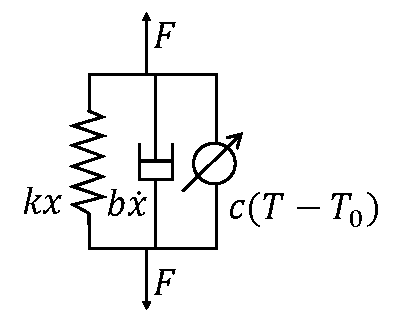
\includegraphics[width=\textwidth]{Model_muscle.pdf}
		\caption{\label{ModelMus}}
	\end{subfigure}
	\begin{subfigure}[t]{0.30\textwidth}
		\centering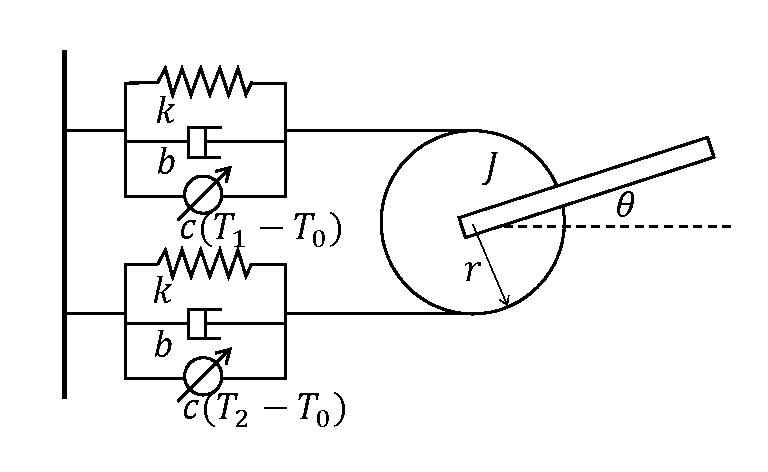
\includegraphics[width=\textwidth]{Model_anta.pdf}
		\caption{\label{ModelAnt}}
	\end{subfigure}
	\begin{subfigure}[t]{0.18\textwidth}
		\centering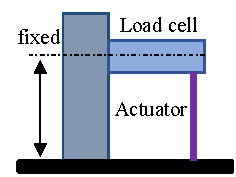
\includegraphics[width=\textwidth]{modeling_static_v2.pdf}
		\caption{\label{static_sch}}
	\end{subfigure}
	\begin{subfigure}[t]{0.18\textwidth}
		\centering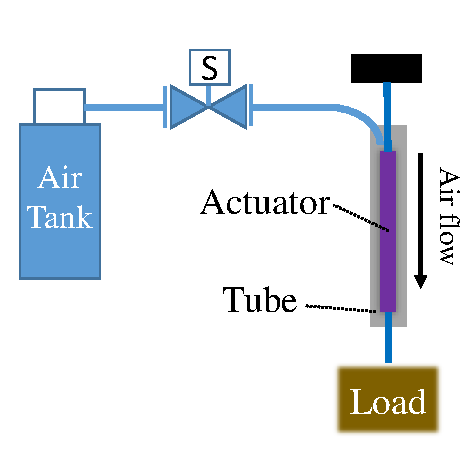
\includegraphics[width=\textwidth]{Static2(v2)_v4.pdf} % An old name of dynamic experiment : static2_v2
		\caption{\label{dynamic_sch}}
	\end{subfigure}
	\caption[Modeling of \scp]{\subref{ModelMus} \scp can be expressed as an combination of a spring, damper, and temperature-dependent system. \subref{ModelAnt} \Anta can be expressed with two complimentary muscles, which change the angular position. \subref{static_sch} Scheme of static experiment. \subref{dynamic_sch} Scheme of dynamic experiment.}
	\label{model+exp_sch}
\end{figure}

\subsection{Static Experiment}
The aim of static experiment was to verify equation \eqref{thermo-mechanical_model} and achieve first and second aim in section \ref{section_aimsappa}. In other words, correlation of \scpnospace's length and tension was investigated at various temperature. 

We can say that muscle have a length $l_{0}$ at ambient temperature with \SI{0}{\newton} tension. Taking $l_{0}$ as standard, we conducted experiments by changing length \SI{15}{\milli\meter} gradually. Also, we used five kinds of voltage - \SI{0}{\volt}, \SI{1.0}{\volt}, \SI{1.8}{\volt}, \SI{2.2}{\volt}, \SI{2.6}{\volt}.

\begin{enumerate}
\item Initial length of \scp was adjusted to $l_0$.
\item We started to apply constant voltage to muscle and waited until muscle's length and temperature becomes steady.
\item When muscle becomes steady, we started recording its physical properties, such as length, tension, temperature, and time.
\item We gradually increased the length of muscle to $l_0+d$.
\item We gradually decreased the length of muscle to $l_0$.
\item End of recording. After cooling to ambient temperature, we repeated 1-5 with other voltage.
\end{enumerate}

Results of static experiment is shown in Fig.\ref{static1_results}. Each of the temperature indicated in legend corresponds to $T_{steady}$. In Fig.\ref{static1_result}, we can observe slight hysteresis. This characteristic graph can be linearly regressed as Fig.\ref{static1_line}. Also, by obtaining force at 10\% strain for each temperature, we can check that force is linearly proportional to $T_{steady}$. (Fig.\ref{static1_dot}) By analyzing graph in Fig.\ref{static1_result}, we got values of $k$, $c$ in \eqref{thermo-mechanical_model}.
\begin{equation}
k=\SI{304}{\newton\per\meter}, c=\SI{0.0501}{\newton\per\degreeCelsius} \notag
\end{equation}

\begin{figure}[t]
	\centering
	\begin{subfigure}[t]{0.3\textwidth}
		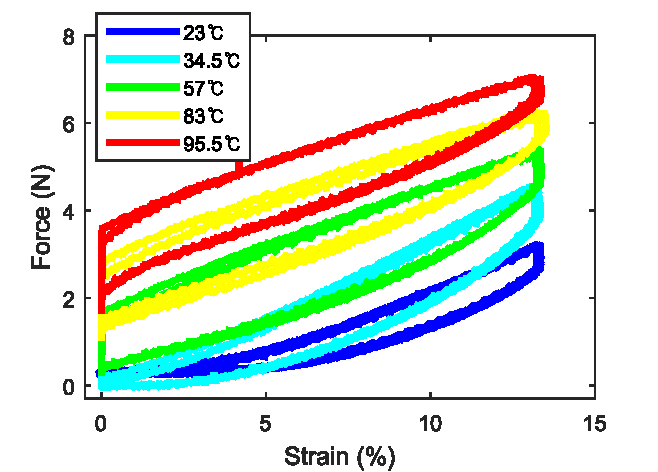
\includegraphics[width=\textwidth]{ForceStrain.pdf}
		\caption{\label{static1_result}}
	\end{subfigure}%
	\begin{subfigure}[t]{0.3\textwidth}
		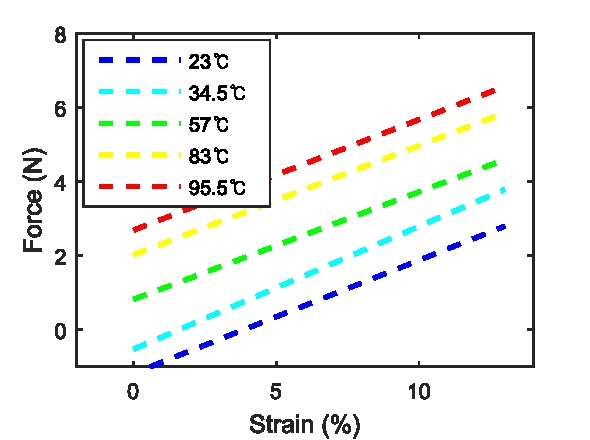
\includegraphics[width=\textwidth]{ForceStrain_line.pdf}
		\caption{\label{static1_line}}
	\end{subfigure}%
	\begin{subfigure}[t]{0.3\textwidth}
		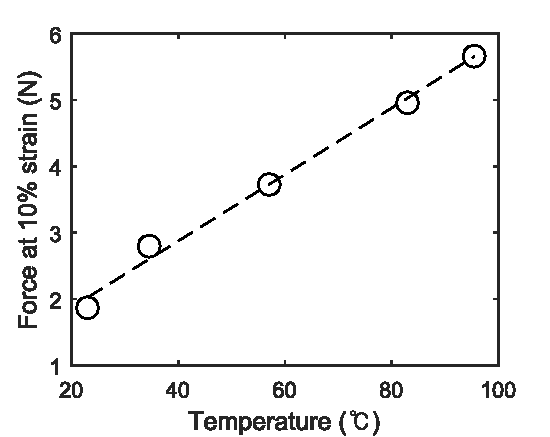
\includegraphics[width=\textwidth]{ForceStrain_dot.pdf}
		\caption{\label{static1_dot}}
	\end{subfigure}
	\caption[Results of static experiment]{\subref{static1_result} Characteristic curves of \scp for various $T_{steady}$. \subref{static1_line} Linear graph of correlation between tension(force) and strain. \subref{static1_dot} Tension is linearly proportional to $T_{steady}$.}
	\label{static1_results}
\end{figure}

\subsection{Dynamic Experiment}\label{section_dynamic} % Important!!
The aim of dynamic experiment was to achieve third to fifth aims in section \ref{section_aimsappa}.
As introduced in section \ref{section_electrical_control}, forced air flow was periodically stopped and resumed to control thermal conductivity of \scpnospace.
This was done by opening the solenoid valve with constant ratio at each period. For example, if we make valve to be opened for \SI{70}{\milli\second} and closed for next \SI{30}{\milli\second}, the ratio is 70\% in this situation. From now on, we will call this as `cooling ratio' and use variable name $r$.
 
%With simple assumption, we can simply guess that $\lambda$ will be proportional to $r$, as equation \eqref{dynamic_simple_model}.
%\begin{equation} \label{dynamic_simple_model}
%\lambda = \lambda_{N}+(\lambda_{F}-\lambda_{N})\cdot r (0\leq r \leq 1)
%\end{equation}
%But, the air flow will keep for a short time right after the valve is closed. Therefore, it is expected that thermal conductivity will be constant if ratio is bigger than $r_{c}$. So, we can modify \eqref{dynamic_simple_model} into \eqref{dynamic_complicated}. 
%
%\begin{equation} \label{dynamic_complicated}
%\lambda = \begin{cases}
%\lambda_{N}+(\lambda_{F}-\lambda_{N})\cdot (r/r_{c}) & r_{c1}<r<r_{c2} \\
%\lambda_{F} & r>r_{c2} \\
%\end{cases}
%\end{equation}

The period of opening and closing was \SI{100}{\milli\second}, which was carefully chosen to get best performance. If the period is too long, thermal conductivity of \scp will periodically change. On the other hand, if the period is too short, the solenoid valve won't perform well because it will take minimal time to open the valve. 

We followed a following process to do dynamic experiment. An Arduino code for dynamic experiment is shown in section \ref{code_dynamic}. We used constant voltage - \SI{2.59}{\volt}. Cooling ratio was variously changed, including $0$(Natural cooling, $\lambda_{N}$), and $1$(Complete forced cooling, $\lambda_{F}$). 
\begin{enumerate}
\item When muscle is begin $T=T_{ambient}$, we started recording time and temperature.
\item Constant power was applied until it reaches steady state.
\item After reaching $T=T_{steady}$, power was disconnected and cooling was started. 
\item When muscle's temperature reaches $T=T_{ambient}$ again, we stopped recording. 
\item We repeated process 1-4 with other voltage and cooling ratio.
\end{enumerate}


\begin{figure}[t]
	\centering
	\begin{subfigure}[t]{0.4\linewidth}
		\centering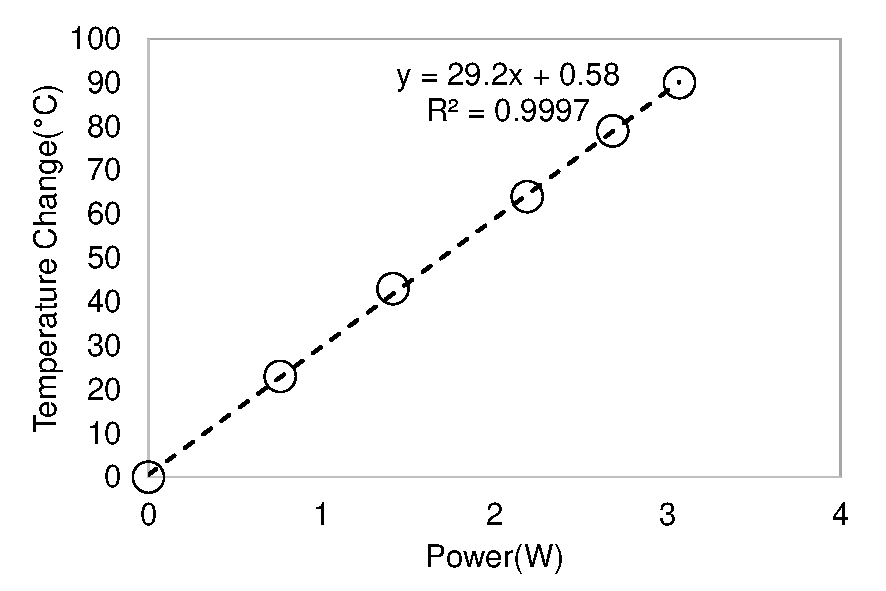
\includegraphics[width=\textwidth]{powerdeltaT-graph_v4.pdf}
		\caption{\label{powerdeltaT}}
	\end{subfigure}%
	\begin{subfigure}[t]{0.4\linewidth}
		\centering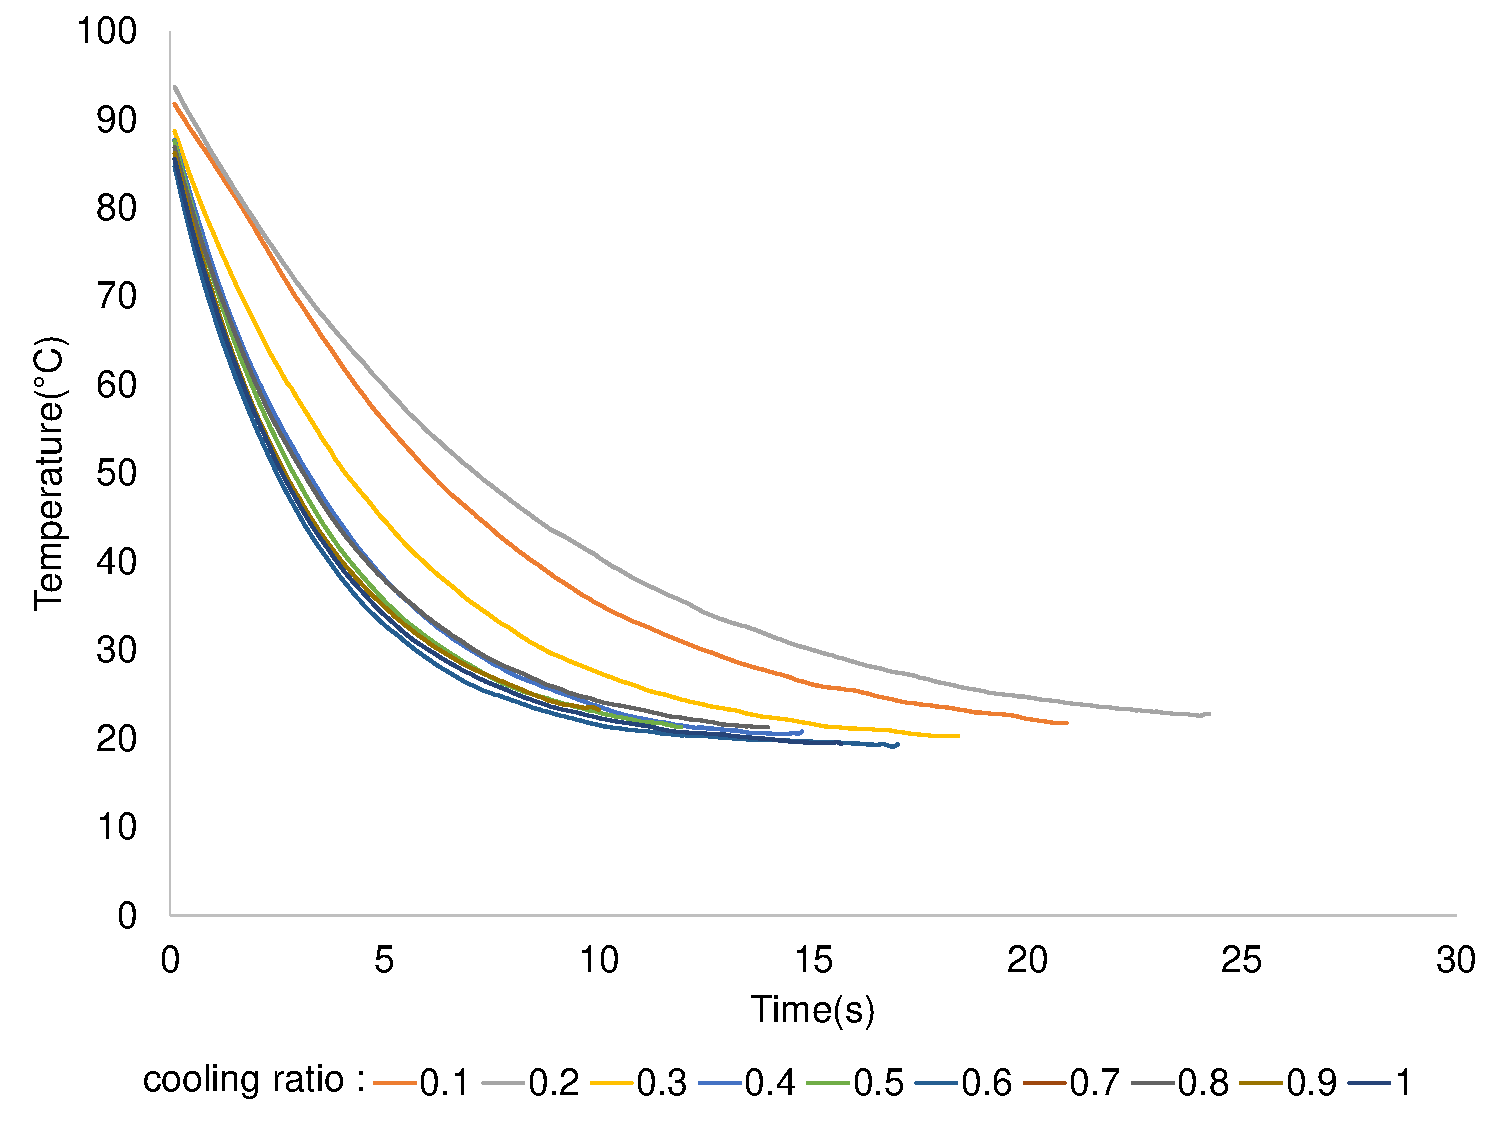
\includegraphics[width=\textwidth]{coolinggraph_v3.pdf}
		\caption{\label{coolinggraph}}
	\end{subfigure}
	\caption[Results of dynamic experiment]{\subref{powerdeltaT} Temperature changes proportionally to power. \subref{coolinggraph} After power was shut down and forced cooling had began, temperature decreased exponentially.}
	\label{result_dynamic}
\end{figure}
%Based on experimental data, we calculated muscle's specific heat $C_{th}$ and thermal conductivity $\lambda$. In detail, we checked that $P$, $\Delta{T}$, $C_{th}$, $\lambda$, and time constant of temperature change $\tau$ satisfies equation \eqref{dynamic_calculation_power} and \eqref{dynamic_calculation_tau}. 

First, by graphing the relation between power $P$ and temperature shift $\Delta{T}=T_{steady}-T_{ambient}$, we could check that they are linearly proportional.
Also, we could check that temperature of \scp changes exponentially as shown in Fig.\ref{coolinggraph}. This was in line with  \eqref{thermo-electrical_model}.

\begin{equation} \label{dynamic_calculation_power}
P = \lambda\Delta{T}
\end{equation}

By applying \eqref{dynamic_calculation_power} into heating graph, we could get $\lambda_{N}$ according to Fig.\ref{powerdeltaT}. Then, by calculating time constant of heating graph, we could calculate \scp system's specific heat $C_{th}$ with \eqref{dynamic_calculation_tau}.\footnote{This was measured three times, resulting \SI{51.3}{\second}, \SI{54.1}{\second}, \SI{53.0}{\second}. Average was \SI{52.8}{\second}.} 

\begin{equation}
\lambda_{N}=\SI{3.42e-2}{\watt\per\degreeCelsius}, C_{th}=\SI{1.81}{\joule\per\degreeCelsius} \notag
\end{equation}

%Meanwhile, as predicted in \eqref{dynamic_complicated}, if $r<0.6$, then $\lambda\propto r$. Else, $\lambda$ was constant, same with $\lambda_{F}$ when $r=1.0$.

Now, we have value of $C_{th}$, so thermal conductivity can be obtained by using \eqref{dynamic_calculation_tau}. Analysis for each cooling graphs is shown in Fig.\ref{analysis_dynamic}.

\begin{equation} \label{dynamic_calculation_tau}
\lambda = \frac{C_{th}}{\tau}
\end{equation}

\begin{figure}[t]
	\begin{subfigure}[t]{0.52\linewidth}
		\centering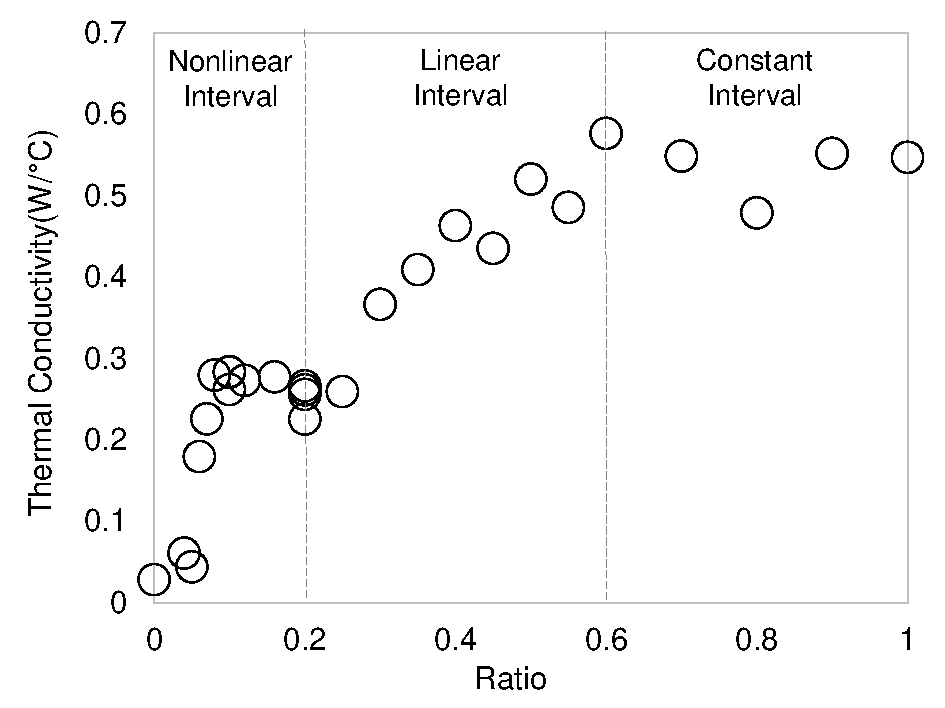
\includegraphics[width=\textwidth]{intervals_v3.pdf}
		\caption{\label{dynamic_proportional}}
	\end{subfigure}%
	\begin{subfigure}[t]{0.39\linewidth}
		\centering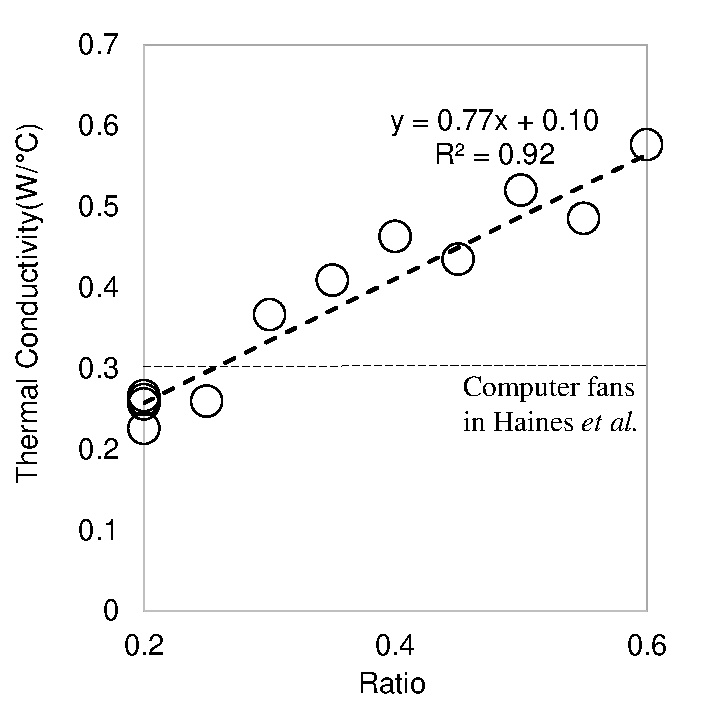
\includegraphics[width=\textwidth]{linear_interval_v4.pdf}
		\caption{\label{linear_interval}}
	\end{subfigure}
	\caption[Analysis of dynamic experiment]{\subref{dynamic_proportional} $\lambda$ was linearly proportional to cooling ratio $r$ when $0.2<r<0.6$.  \subref{linear_interval} $\lambda$ can be calculated with equation \eqref{lambda_control}.}
	\label{analysis_dynamic}
\end{figure}

In Fig.\ref{dynamic_proportional}, we could observe that thermal conductivity in function of $r$ can be divided into three parts - nonlinear, linear, and constant interval. If $r<0.2$, $\lambda$ rapidly increased near $r=0.1$. Also, $\lambda$ doesn't increased anymore if $r>0.6$, {\it i.e.} $\lambda = \lambda_{F}$. This can be also observed from cooling graph in Fig.\ref{coolinggraph}.
Therefore, the linear interval was chosen for \Apcnospace.(Fig.\ref{linear_interval}) The thermal conductivity in controllable(linear) interval was usually higher than cooling by computer fans, which were used by Haines \etalspace and determined to be $\lambda_{fan}=\SI{0.30}{\watt\per\degreeCelsius}$.

\begin{equation} \label{lambda_control}
\lambda = 0.77\cdot r + 0.10 (\si{\watt\per\degreeCelsius}), 0.2\leq r \leq 0.6
\end{equation}


%Meanwhile, we have to justify the approximation used in section \ref{section_dynamic_appa}. 
Meanwhile, we have to check that the load used in dynamic experiment doesn't effected muscle's thermal power. % (?)
Total electrical power of muscle is about $(\SI{1.0}{\volt})^2/(\SI{2.5}{\ohm})=\SI{0.4}{\watt}$, cooling speed is about $\SI{1.39}{\joule\per\degreeCelsius} \cdot \SI{1}{\degreeCelsius\per\second}=\SI{1.39}{\watt}$ while gravitational power is about  $\SI{0.4}{\kilo\gram} \cdot  \SI{9.8}{\meter\per\second\square} \cdot \SI{0.001}{\meter\per\second}=\SI{0.004}{\watt}$. So we can conclude that load didn't affected on measurement of muscle's thermal properties.



